\section{Domain analysis and model}\label{sec:domain}
\phantomsection

Domain analysis
\subsection{System Requirements}

\subsection{Medical Analysis}
\subsubsection{Difference between snoring and Sleep Apnea disorder}
Sometimes snoring and Sleep Apnea are used interchangeably, but from the medical point of view the terms represent different concepts. For the sake of being accurate, it is absolutely necessary to define each of them.

Snoring is the vibration of respiratory structures and the resulting sound. It is caused by the obstructed air movement during breathing while sleeping. From the intuitive point of view, snoring is simple to imagine and even mimic. This noisy, rough sound is created from the vibrations of uvula and soft palate. Uvula and soft palate are presented in Figure \ref{fig:uvula_and_soft_palate}.

\begin{figure}[!ht]
\centering
\includegraphics[scale=0.5]{01_uvula_and_soft_palate.jpg}
\caption{Uvula and soft palate}
\label{fig:uvula_and_soft_palate}
\end{figure}

% \begin{figure}[!ht]
% \centering
% \includegraphics[width=13cm]{iter}
% \caption{Iterative and Incremental Development, \cite{Larman2}}\label{IterativeAndIncremental}
% \end{figure}


Even though snoring is common among people of all ages, the whole issue stays relatively undiagnosed and poorly researched. The primary reason might be the fact that snoring itself isn't harmful. A person snoring during his sleep, might be perfectly healthy with no disorders whatsoever. Nevertheless snoring remains to be a social problem for people who share a bed. The sleeping partner can develop sleep difficulties in such cases.

The causes of snoring might be:
\begin{itemize}[topsep=5pt, partopsep=0pt,itemsep=3pt,parsep=1pt]
 \item throat weakness, which causes the throat to close during sleeping;
 \item being overweight - the fat around the neck puts pressure on the airways;
 \item nose blockage caused by crooked, bent or deformed nasal septum (the structure that separates the nostrils);
 \item abnormalities in the bones of the face, like the mispositioned jaw;
 \item nasal polyps;
 \item stuffed nose during cold and allergies;
 \item consumption of relaxants like drugs or alcohol at bedtime;
 \item position during sleep, which may result in dropping one's tongue in the back of the mouth.
\end{itemize}

Snoring itself is not dangerous, but can lead to several minor life discomforts, like daytime drowsiness, lack of a partner due to its psychosocial impact, decreased libido, lack of focus.

The real risks come up when talking about Sleep Apnea. It is a serious disorder in which one can have one or more pauses in breathing or shallow breaths while sleeping. The pauses in breathing are called apneas and can last from few seconds to several minutes. The shallow breathing event is called hypopnea. 

There are different types of Sleep Apnea:
\begin{enumerate}[topsep=5pt, partopsep=0pt,itemsep=3pt,parsep=1pt]
 \item Central Sleep Apnea (CSA) - breathing is interrupted by a lack of respiratory effort;
 \item Obstructive Sleep Apnea (OSA) - breathing is interrupted by a physical block to the airflow despite respiratory effort;
 \item Mixed Sleep Apnea (MSA) - contains properties from both types of Sleep Apnea.
\end{enumerate}

CSA is associated with a number of different neurological problems, when during sleep brain signals that tell the body to breath don't work properly. Respectively no effort is made to inhale as expected. Typically CSA is not associated with any snoring, therefore its detection and diagnosis goes beyond the scope of this work. In contrast in case of OSA an effort to breath is made, but because of the collapse of the upper airway, air doesn't get into the lungs.

% !!! REFERENCE
According to [1] CSA is the most rarely met and constitutes 0.4\% prevalence. Mixed or Complex Sleep Apnea is met 15\% of times. The most often is OSA - 84\%. Therefore OSA represents the most curious and interesting type of Sleep Apnea disorder, and it is the type that causes snoring due to the air squeeze past the blockage. 

Sleep Apnea is also characterized by the frequency of apneas. There exists 2 indexes can measure Sleep Apnea objectively: 
\begin{itemize}[topsep=5pt, partopsep=0pt,itemsep=3pt,parsep=1pt]
 \item Apnea Hypopnea Index (AHI) - total number of apneas and hypopneas during an hour;
 \item Respiratory Disturbance Index (RDI) - total number of apneas, hypopneas and respiratory-effort related arousals (RERAs) during an hour.
\end{itemize}

The AHI and RDI can tell the severeness of OSA. Mild OSA ranges from 5 to 14.9 events per hour, moderate OSA - from 15 to 29.9 events per hour of sleep and severe OSA means having over 30 events per hour of sleep. The following formalization is disputable, since the diagnosis of OSA must include also a series of other factors about the patient, like age, blood saturation, heart rate.

As well as mere snoring, OSA is caused most often by structural features, low muscle tone and soft tissue around the airway. The risk of being diagnosed rises with age, increased body weight and active smoking. Indeed elderly people are more likely to have OSA. Normally men are more exposed to the disorder than women or children. Though is it not uncommon for children to suffer from OSA and manifest snoring during night. 

% !!! REFERENCE
According to “National Heart, Lung, and Blood Institute”[2] most common symptoms of sleep apnea are:
\begin{itemize}[topsep=5pt, partopsep=0pt,itemsep=3pt,parsep=1pt]
 \item loud snoring;
 \item waking up with a very dry sore or dry throat;
 \item occasionally waking up with a choking or gasping sensation;
 \item sleepiness and lack of energy during the day;
 \item restless sleep;
 \item sleepiness during driving;
 \item forgetfulness, mood changes, irritability, anxiety and depression;
 \item morning headaches.
\end{itemize}

Most of the signs of OSA are vague and hard to measure. Many of those can be caused by tens of different physical and psychological disorders. Therefore the most obvious is load and chronic snoring.

Here is a simple illustration of a man sleeping without obstruction (Figure \ref{fig:sleep_without_obstruction}) and with obstruction (Figure \ref{fig:sleep_with_obstruction}). Blue arrow indicate oxygen flow, orange arrows - carbon dioxide flow.

\begin{figure}[!ht]
\centering
\includegraphics[scale=0.4]{02_sleeping_without_obstruction.png}
\caption{Sleeping without obstruction}
\label{fig:sleep_without_obstruction}
\end{figure}

\begin{figure}[!ht]
\centering
\includegraphics[scale=0.4]{03_sleeping_with_obstruction.png}
\caption{Sleeping with obstruction}
\label{fig:sleep_with_obstruction}
\end{figure}

By defining both terms, it is possible now to see the differences between two and to establish a strong correlation between OSA and snoring. In simple words, it is clear that not any snoring is caused by OSA and almost every OSA patient will suffer from snoring during sleep.

\subsubsection{Risks and diagnosis of Obstructive Sleep Apnea disorder}
As it was stated above Obstructive Sleep Apnea is a rather serious disorder. Although a very minor degree of OSA is considered not dangerous and within the limits of normal sleep. The other small percentage of people with OSA are in the risk zone.

Firstly OSA can lead to high blood pressure. The following is explained by the fact that nighttime waking causes the hormonal system to go into overdrive. Additionally the reduction in blood oxygen saturation that happens due to the pauses in breathing, also can cause elevated arterial pressure (hypertension).

The most serious consequence of OSA is considered the heart disease. On average people with sleep apnea have 30\% higher risk of having a heart attack than those who don't have OSA. Chronic sleep apnea can cause congestive heart failure, called cor pulmonale. Speaking in simple terms, low oxygen level and midnight waking stress lead to strokes and atrial fibrillation.

It is known that 80\% of diabetics have OSA. Thought a direct link between the two was never proved, studies show that sleep deprivation causes insulin resistance. 

Same strange link between OSA and asthma exists. If sleep apnea is being treated, than patients report a decrease in asthma attacks. 

Previously it was stated that obesity is a cause for sleep apnea and two thirds of people suffering from OSA are extremely overweight. Obesity in this case act also as a consequence of sleep apnea, because it impairs the endocrine system of the human body, causing the release of the hormone ghrelin, which makes people crave carbohydrates and sweets. Moreover OSA can caused lower metabolism, because of the patient feeling sleepy and tired. Consequently it is necessary to treat OSA first, in order to feel better, be active and do exercises to lose weight.

% !!! REFERENCE
Car accidents are a very important consequence of untreated OSA. Several studies [4] and [5] show the same results - people with sleep apnea syndrome have an increased risk of automobile accidents. Patients with sleep apnea often report falling asleep while driving as least once per week. Generally impaired drivers with Sleep Apnea may cause many auto accidents. 

% !!! REFERENCE
According to Morbidity and Mortality Weekly Report from Centers for Disease Control and Prevention[3] drowsy driving has been responsible for an estimated 1500 fatalities and 40000 nonfatal injuries annually in the United States. Populations previously found at greatest risk included persons aged 16--29 years (particularly males), those with untreated sleep apnea syndrome or narcolepsy, and those who work shifts, particularly night shifts or extended shifts.

% !!! REFERENCE
Some of the latest statistics [6] claim that 5\% of all people have sleep apnea disorder. 37.9\% unintentionally fell asleep during the day at least once per month and 4.5\% nodded off or fell asleep while driving in the last month.

There are several ways to diagnose sleep apnea. Normally it should be a quintessential analysis of clinical symptoms and some formal sleep investigations. Clinical symptoms include daytime sleepiness, anxiety, fatigue and others discussed earlier. The formal sleep study can be conducted in the lab or at home. 

Polysomnography is the most complex sleep study. It involved a multi-parametric test that records biophysiological changes that occur during sleep. The result of this test is called Polysomnogram (PSG). A PSG will record heart rhythm, brain activity (EEG), eye movements (EOG), muscle activity and skeletal muscle activation (EMG). 

Usually the patient comes to the sleep lab and is wired up to multiple sensors that are attached to multiple channels of data. During the night a technician observes sleep activity by looking at the monitors and computers screen, that displays all the data. Consequently all the recorded data will be analysed manually by specialists in the field.

Polysomnographic test can be conducted also at home. Sophisticated home studies can give the same accuracy, but are quite complex and time consuming to set up for self monitoring. That is the reason why special screening tools are used for home-based test. Special equipment is given to the patient. Usually it consists of an thermistor (airflow measuring device) and a pulse oximeter (blood oxygen monitoring device). The patient would sleep at home with the device and after one or more nights will return it to the physician. 

In case of sleep apnea polysomnographic test characterizes pauses in breathing. These pauses are followed by a relative decrease in blood oxygen and an increase in the blood carbon dioxide. In case of CSA there are no chest movements whatsoever, but in case of OSA - the movements typically become even more pronounced. Based the results of polysomnographic test, AHI is deducted. 

\begin{figure}[!ht]
\centering
\includegraphics[width=13cm]{04_oximeter.jpg}
\caption{Oximeter}
\label{fig:oximeter}
\end{figure}

For non-invasive method of monitoring blood oxygenation an oximeter (Figure \ref{fig:oximeter}) is being used. Howether an oximeter doesn't measure any apneic events or respiratory event-related arousals, hence doesn't produce any AHI value.

Lately all sorts of gadgets and devices started to appear to measure sleep apnea. There exists a big variety of portable monitors available on the market. Here is a classification of PSG types by American Academy of Sleep Medicine and novel devices.

\begin{figure}[!ht]
\centering
\includegraphics[width=13cm]{05_psg_classification.jpg}
\caption{PSG classification}
\label{fig:psg_classification}
\end{figure}

% !!! REFERENCE
Full overnight polysomnographic test is considered the golden standard - type I. Most of the portable monitors are of type III and IV [8]. Even though portable monitors start gaining in attention, their proper usage is more challenging and the interpretation of results more vague.

In conclusion OSA is a serious disorder that should be treated as soon as possible, because it can lead to some unwanted consequences. There are many ways to identify OSA by consulting a doctor and taking a PSG test. The main gap that exists in problem solving is how do people suspect that they have OSA and decide to pay a visit to the doctor. This is the question that the following work is trying to clear up.

\subsubsection{Treatment of Obstructive Sleep Apnea disorder}
There are different ways to treat OSA depending on the severeness of the disorder. Firstly the patient will be asked to quit smoking, avoid alcohol and any other medicamentation that relax the central nervous system. If the patient is overweight, it is a good idea to lose some weight. Generally physical exercises will improve sleep apnea. If it's possible the patient should sleep on the side as opposed to sleeping on the back. Meanwhile the patient can use special anti-snoring sleeping pillows, that keep the head aligned to the body without dropping it too much in the back or to the front. Very often the elevated position helps prevent the gravitational collapse of the airway. All those solutions are simple, straightforward and don't require any serious medical intervention.

Possibly physical intervention for curing OSA is the most popular one. Positive airway pressure is the technique where a breathing device pumps a controlled stream of air through a mask worn over the nose, mouth or both. The idea behind the positive airway pressure is simple - it keeps the relaxed areas open.  There are a bunch of variations of positive airway pressure devices:
\begin{itemize}
 \item CPAP (Continuous Positive Airway Pressure) - a device that continuously pumps air to the nose and mouth;
 \item VPAP (Variable Positive Airway Pressure) - a more sophisticated device that controls the stream of air. It pumps a higher pressure of air on inhalation and a lower pressure on exhalation. It can be used when patients have problems exhaling against an increased pressure airflow;
 \item APAP (Automatic Positive Airway Pressure) - the functional part is similar to previous examples, but uses a bunch of sensors to continuously monitor patient's breathing;
 \item Nasal EPAP (Expiratory Positive Airway Pressure) - uses person's breath to create the pressure.
\end{itemize}

CPAP (Figure \ref{fig:cpap}) in comparison with many oral appliances is considered the most effective device for preventing sleep apnea. Mandibular advancement splint is an oral appliance that shifts the lower jaw forward and opens the bite slightly. This kind of specially fabricated appliances are efficient for people with mild or average form of sleep apnea.

\begin{figure}[!ht]
\centering
  \includegraphics{06_cpap.jpg}
\caption{CPAP - Continuous Positive Airway Pressure}
\label{fig:cpap}
\end{figure}

The usage of medicamentation was never proved to be effective in case of sleep apnea treatment. Usually Central Sleep Apnea can be treated with such drugs as acetazolamide, zolpidem and triazolam.

Surgery is also an alternative option to reduce severe sleep apnea. Even though surgery doesn’t give any guarantees to free up the patient from OSA and the evidence for all types of sleep surgery is quite poor. 

Some of the common types of surgeries are:
\begin{itemize}
 \item tonsillectomy and/or adenoidectomy;
 \item removal or the reduction of uvula and soft palate;
 \item nasal surgery, like turbinectomy or straightening of nasal septum;
 \item reduction of tongue base;
 \item moving the jaw a little bit up front and pulling the tongue away from the back of the airway;
 \item maxillomandibular advancements.
\end{itemize}

Some of those surgeries can be conducted using Radiofrequency ablation (RFA). It uses low frequency radio wave energy to target tissue, causing coagulative necrosis. It is less common than CPAP or classical surgery, but has potential to become one.

% [Can be extended]

Those have been all the popular and most common ways to treat sleep apnea disorder. Neither of them gives absolute guarantee for a apnea-free life, but there exists a choice to make between invasive and non-invasive solutions. 

\subsection{Theoretical Analysis}
\subsubsection{Digital signal processing}
In the context of communication everything is a wave. This is the starting point to understanding that everything travels as a wave and can be represented graphically. Signals can be analog and discrete. Discrete-time signals consist of sequences of quantities. In case it is obtained from a continuous-time signal it is characterized by a sampling rate. The process of analog to digital conversion consists of 2 step process: quantization and discretization. If both time series and the amplitude of a signal were discretized, then it is a digital signal.

Digital signal processing (further used as DSP) represents a very important part in signal analysis. Since the major goal of this thesis is to develop an automated method for snore detection, digital signal processing becomes critical for correct computations. Roughly it might be considered a preprocessing phase in snore recognition, which is applied before feature extraction and machine learning. 

DSP is the mathematical manipulation of signal information represented in discrete domain: time, frequency. One type of such signal represents the sound of which we are particularly interested. Generally the aim of DSP is to improve the accuracy and reliability of discrete signals by eliminating or diminishing noise.

For the sake of clarity there will be presented a simple signal to which all the relevant digital processing algorithms will be applied.

First it is necessary to generate a sample wave. For the matter of simplicity the signal is generated using 2 sine waves as shown in Formula \eqref{eq:sample_sine}. The result is displayed in Figure \ref{fig:sines}. The lower plot shows the same signal as on the upper plot, plus some random normally distributed noise. Further we will use the noisy data to do preprocessing.

\begin{equation} \label{eq:sample_sine}
 y(t) = \sin(2\pi 0.05 x) + 3\sin(2\pi 0.09 x)
\end{equation}


\begin{figure}[!ht]
\centering
  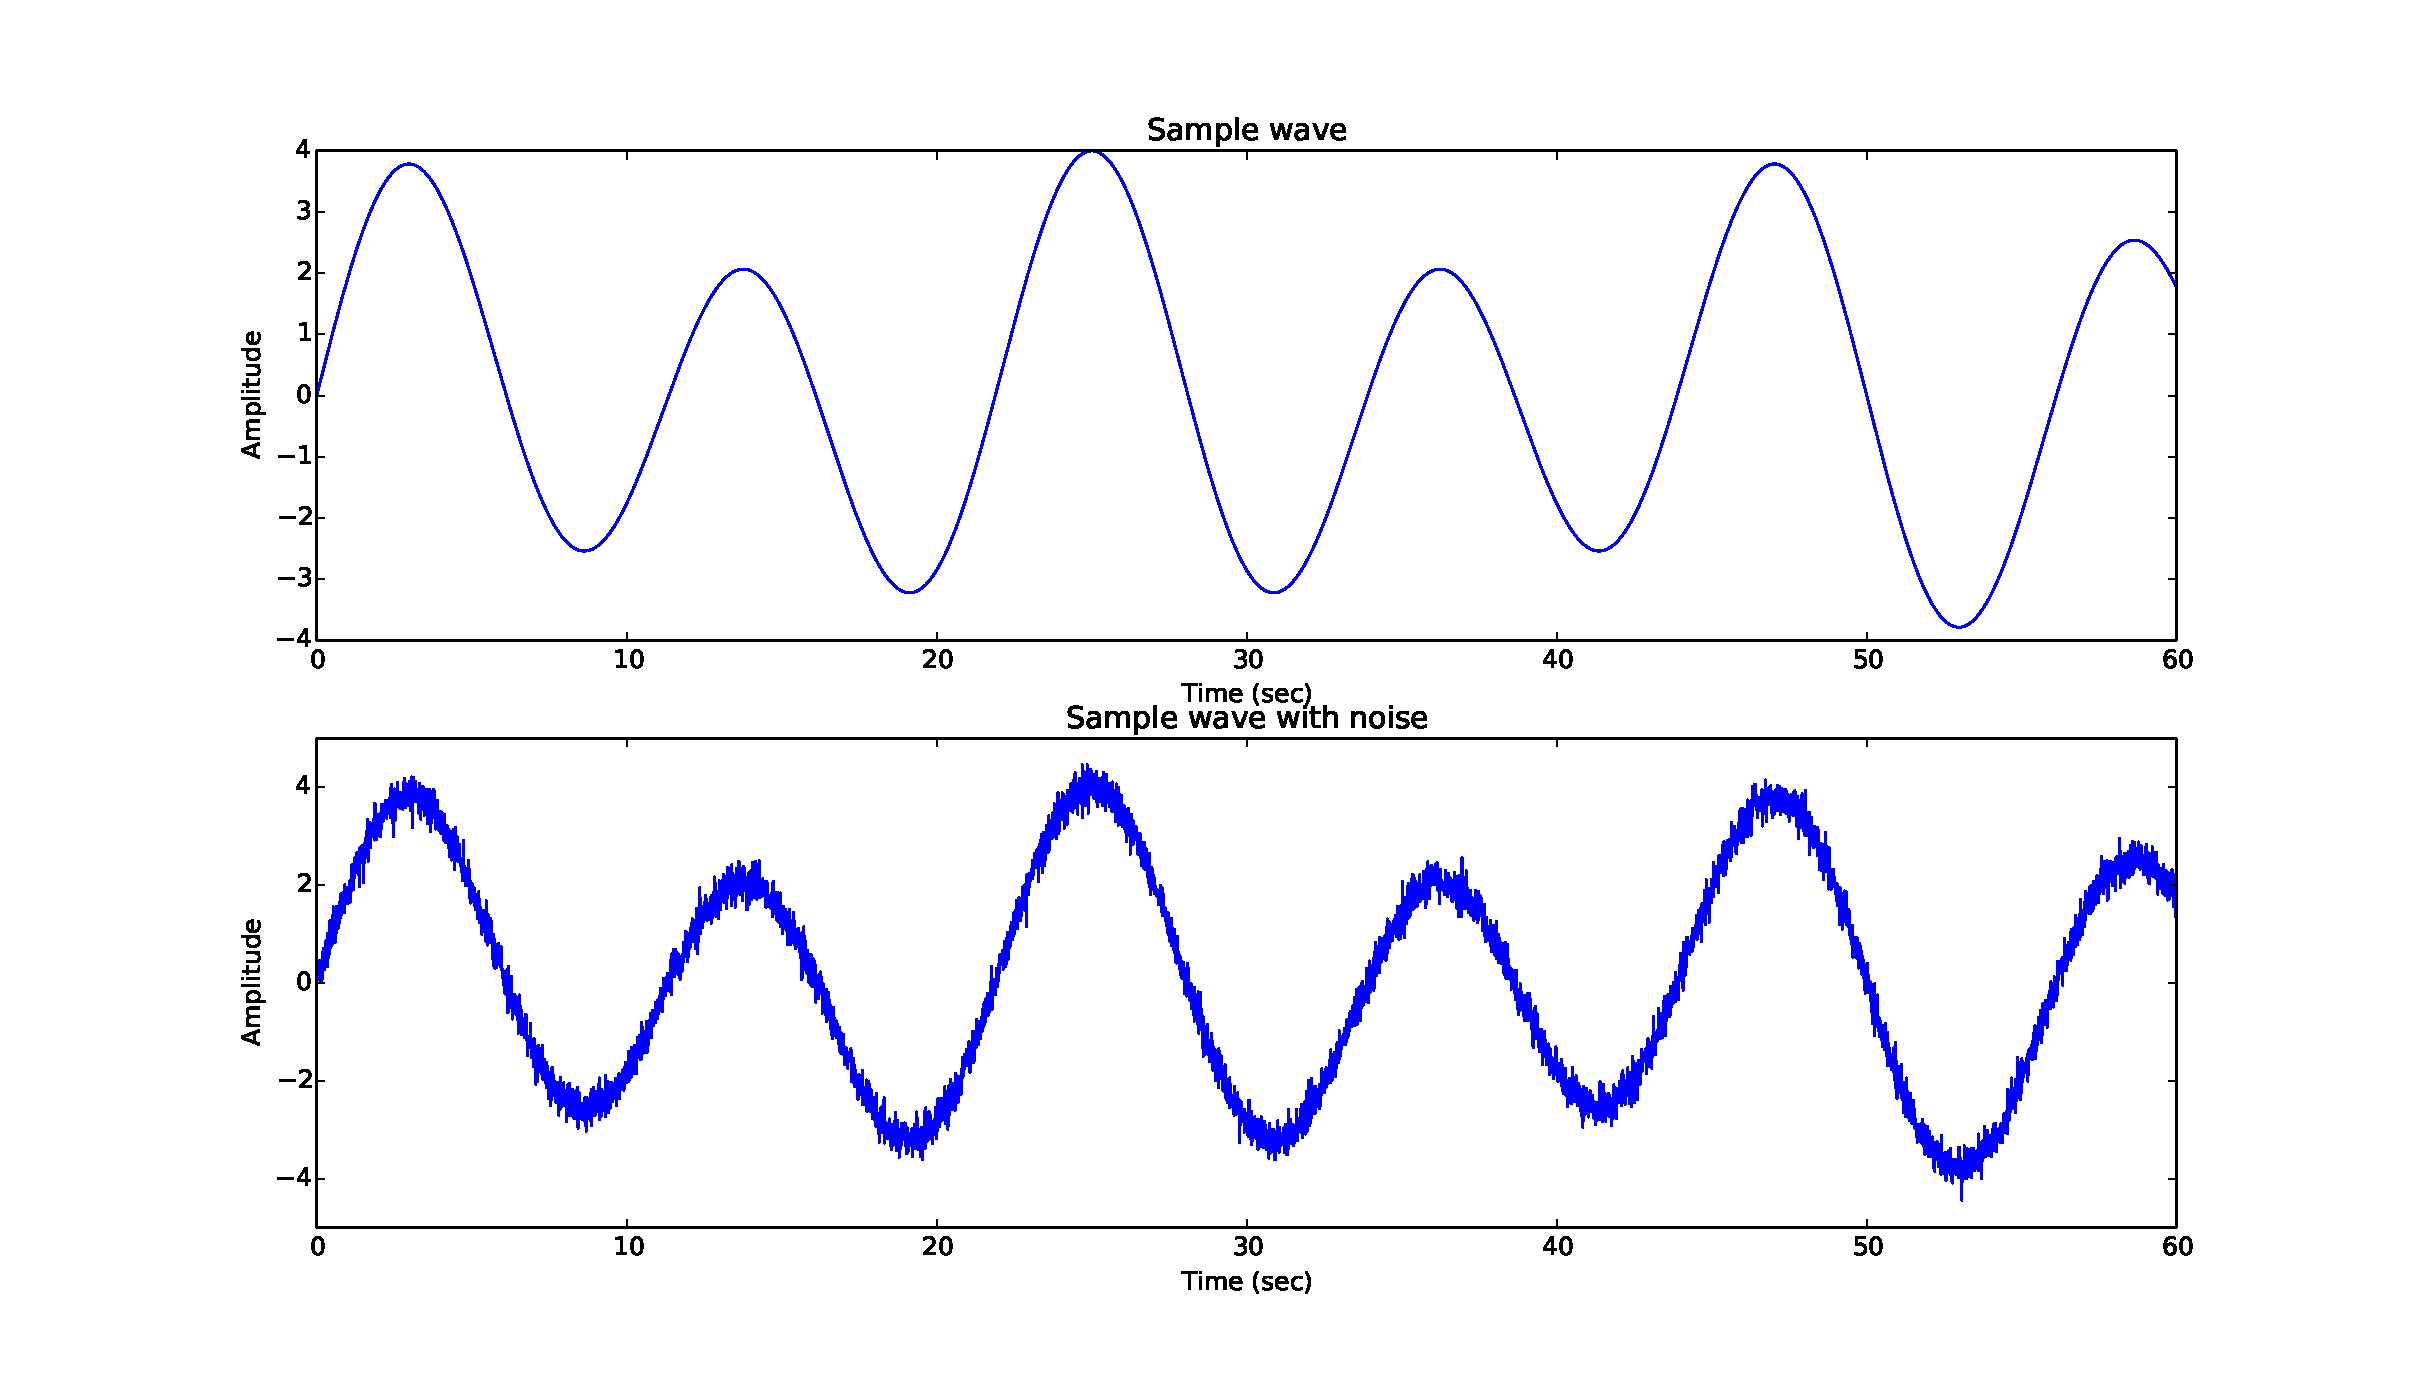
\includegraphics[width=15cm]{07_sine_wave.eps}
\caption{Sample sine waves with and without noise}
\label{fig:sines}
\end{figure}

The most common way to improve the quality of a signal is to use digital filtering. It mainly consists of mathematical manipulations of a number of adjacent samples to a current sample. In preprocessing phase a low-pass filter is being used. It attenuates the high frequencies and passes low frequencies. It is characterized by the cut-off frequency, which should be specified explicitly for each signal. Low-pass filtering will make the signal appear smoother by removing short-term fluctuations. 

In this particular case the low-pass filter is implemented using Butterworth filter -- it has maximally flat frequency response in the passband. Butterworth filter introduces a phase shift between the original and filtered signal. In digital implementation the lag can be ignored, because the filtering happens twice, once forward and once backward. Second order 'lowpass' type filter is created for filtering the signal in this particular case. For the signal generated earlier the cutoff frequency is $10$. The results of filtering can be viewed in Figure \ref{fig:lowpass}.

\begin{figure}[!ht]
\centering
  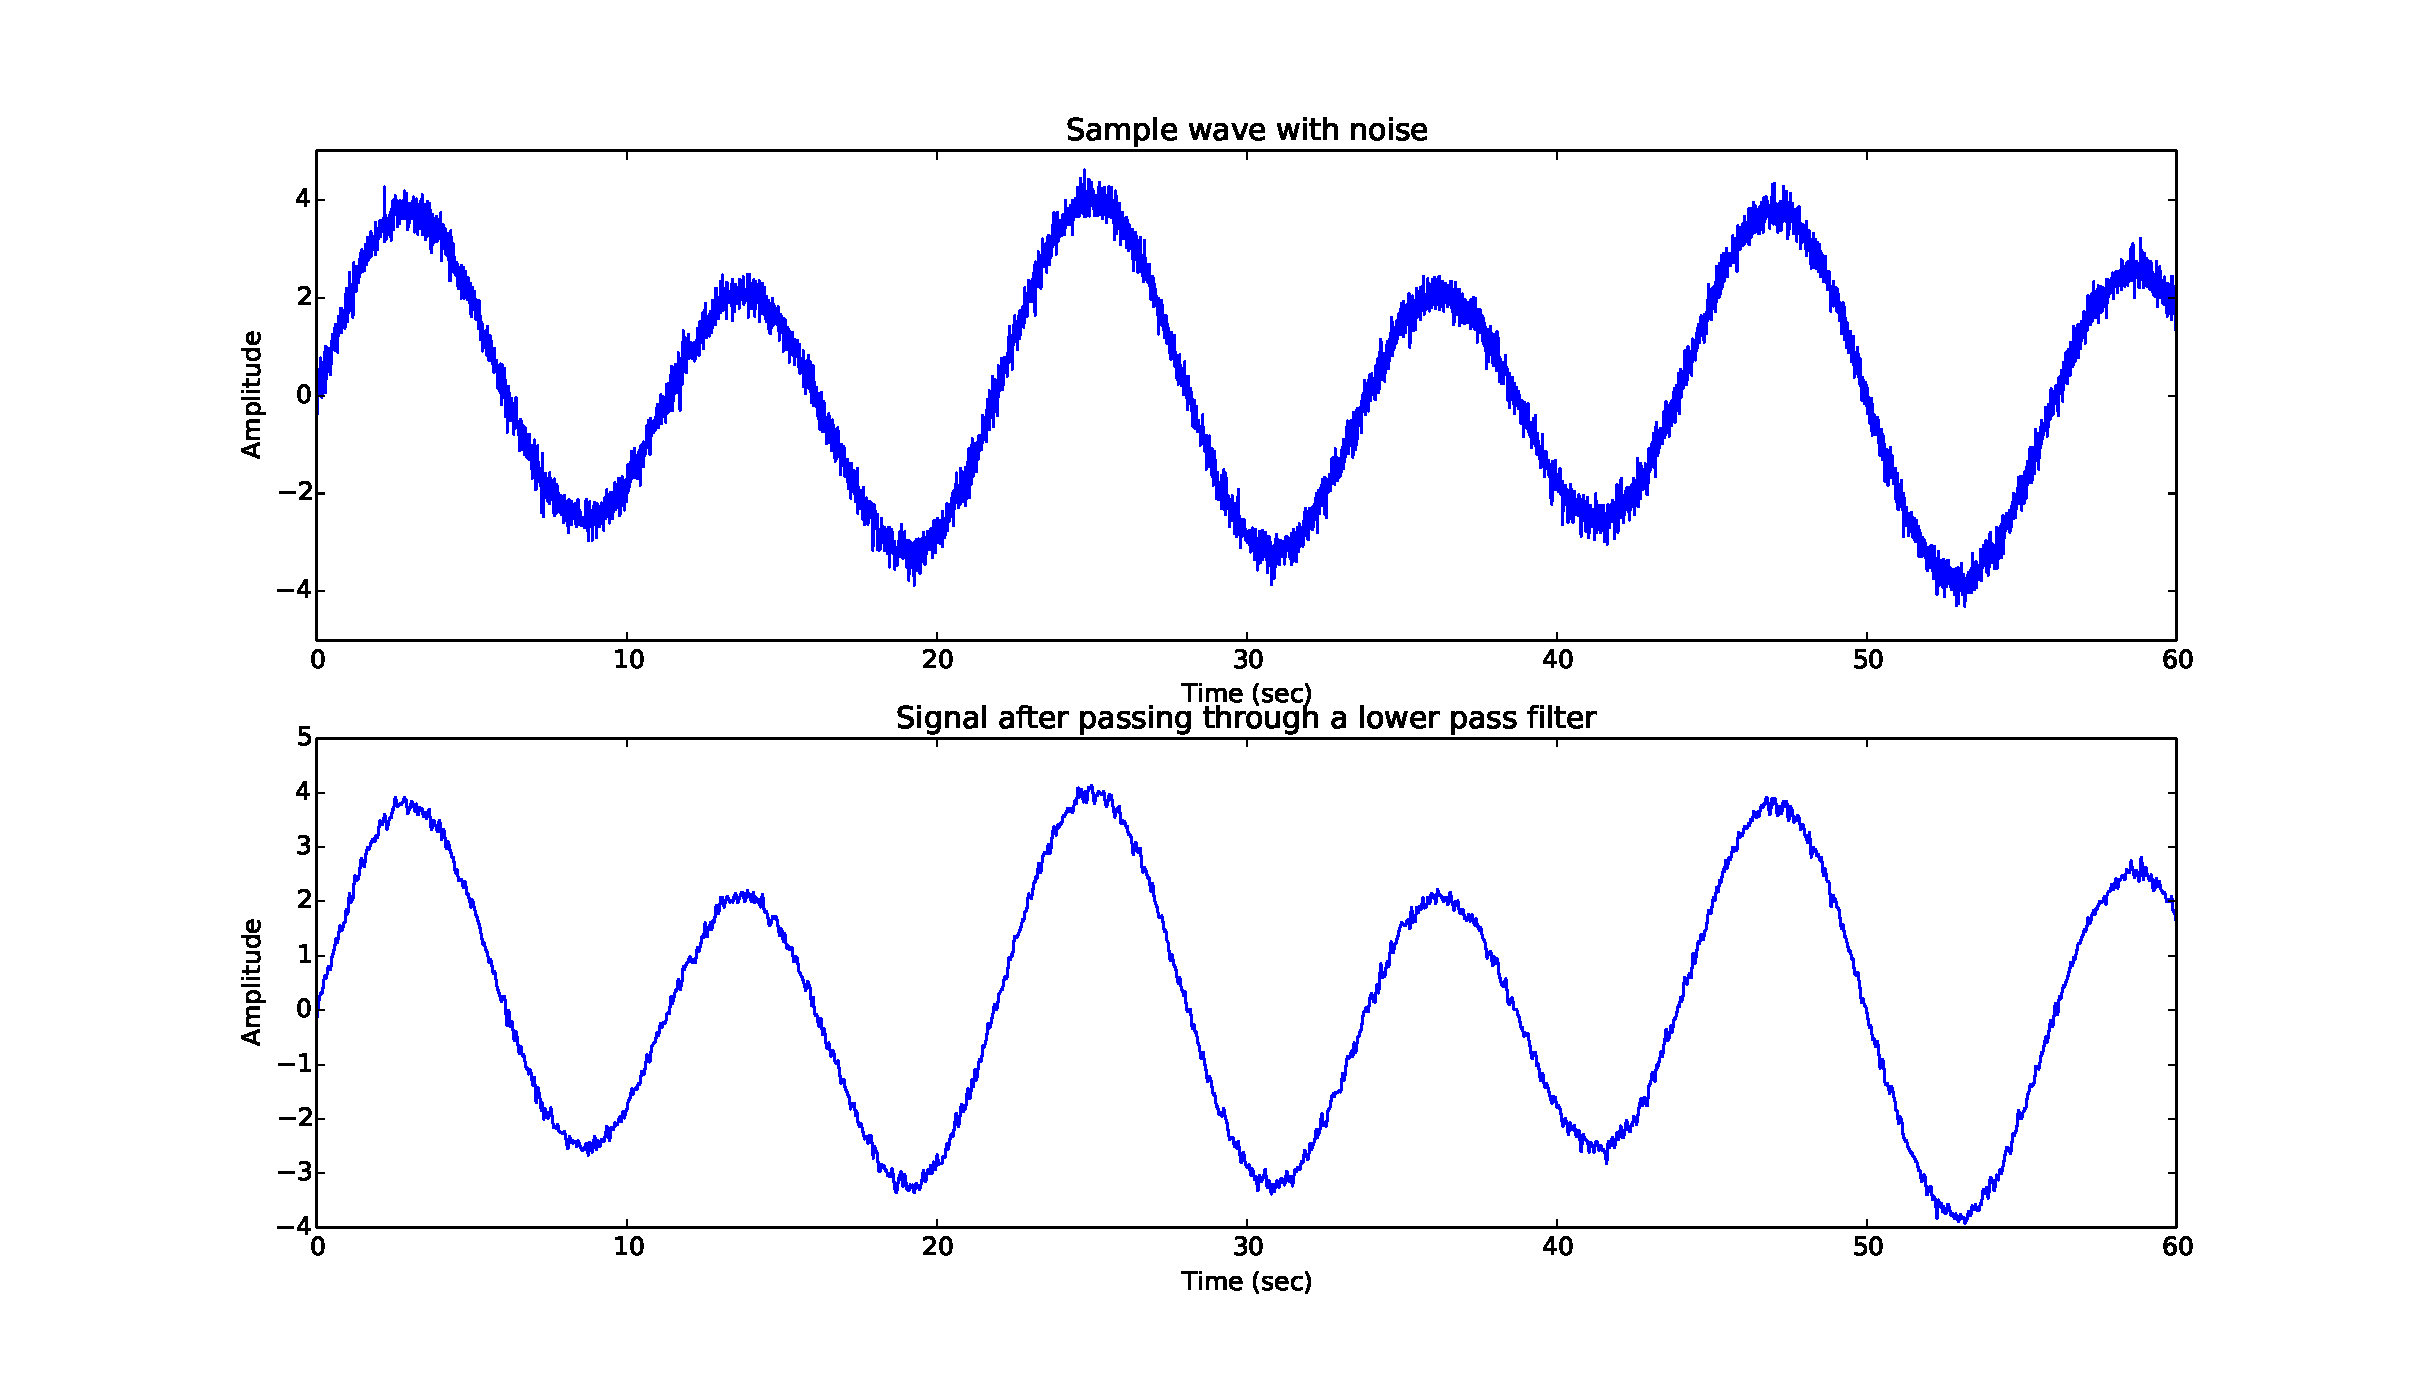
\includegraphics[width=15cm]{08_lowpass.eps}
\caption{Sine wave with noise before and after low-pass filtering}
\label{fig:lowpass}
\end{figure}

From the resulted data, it is easy to see that signal becomes smoother and doesn't contains high frequencies. Mathematically and intuitively it gives a good-enough result. 

The next step is to perform normalization \eqref{eq:normalization}.

\begin{equation} \label{eq:normalization}
 x = \frac{x - \overline{x}}{\sigma}
\end{equation}

where $\overline{x}$ represents the arithmetic mean and $\sigma$ is the standard deviation. 

Consequently the signal wave is normalized and an example of normalization can be viewed in Figure \ref{fig:normalized}.

\begin{figure}[!ht]
\centering
  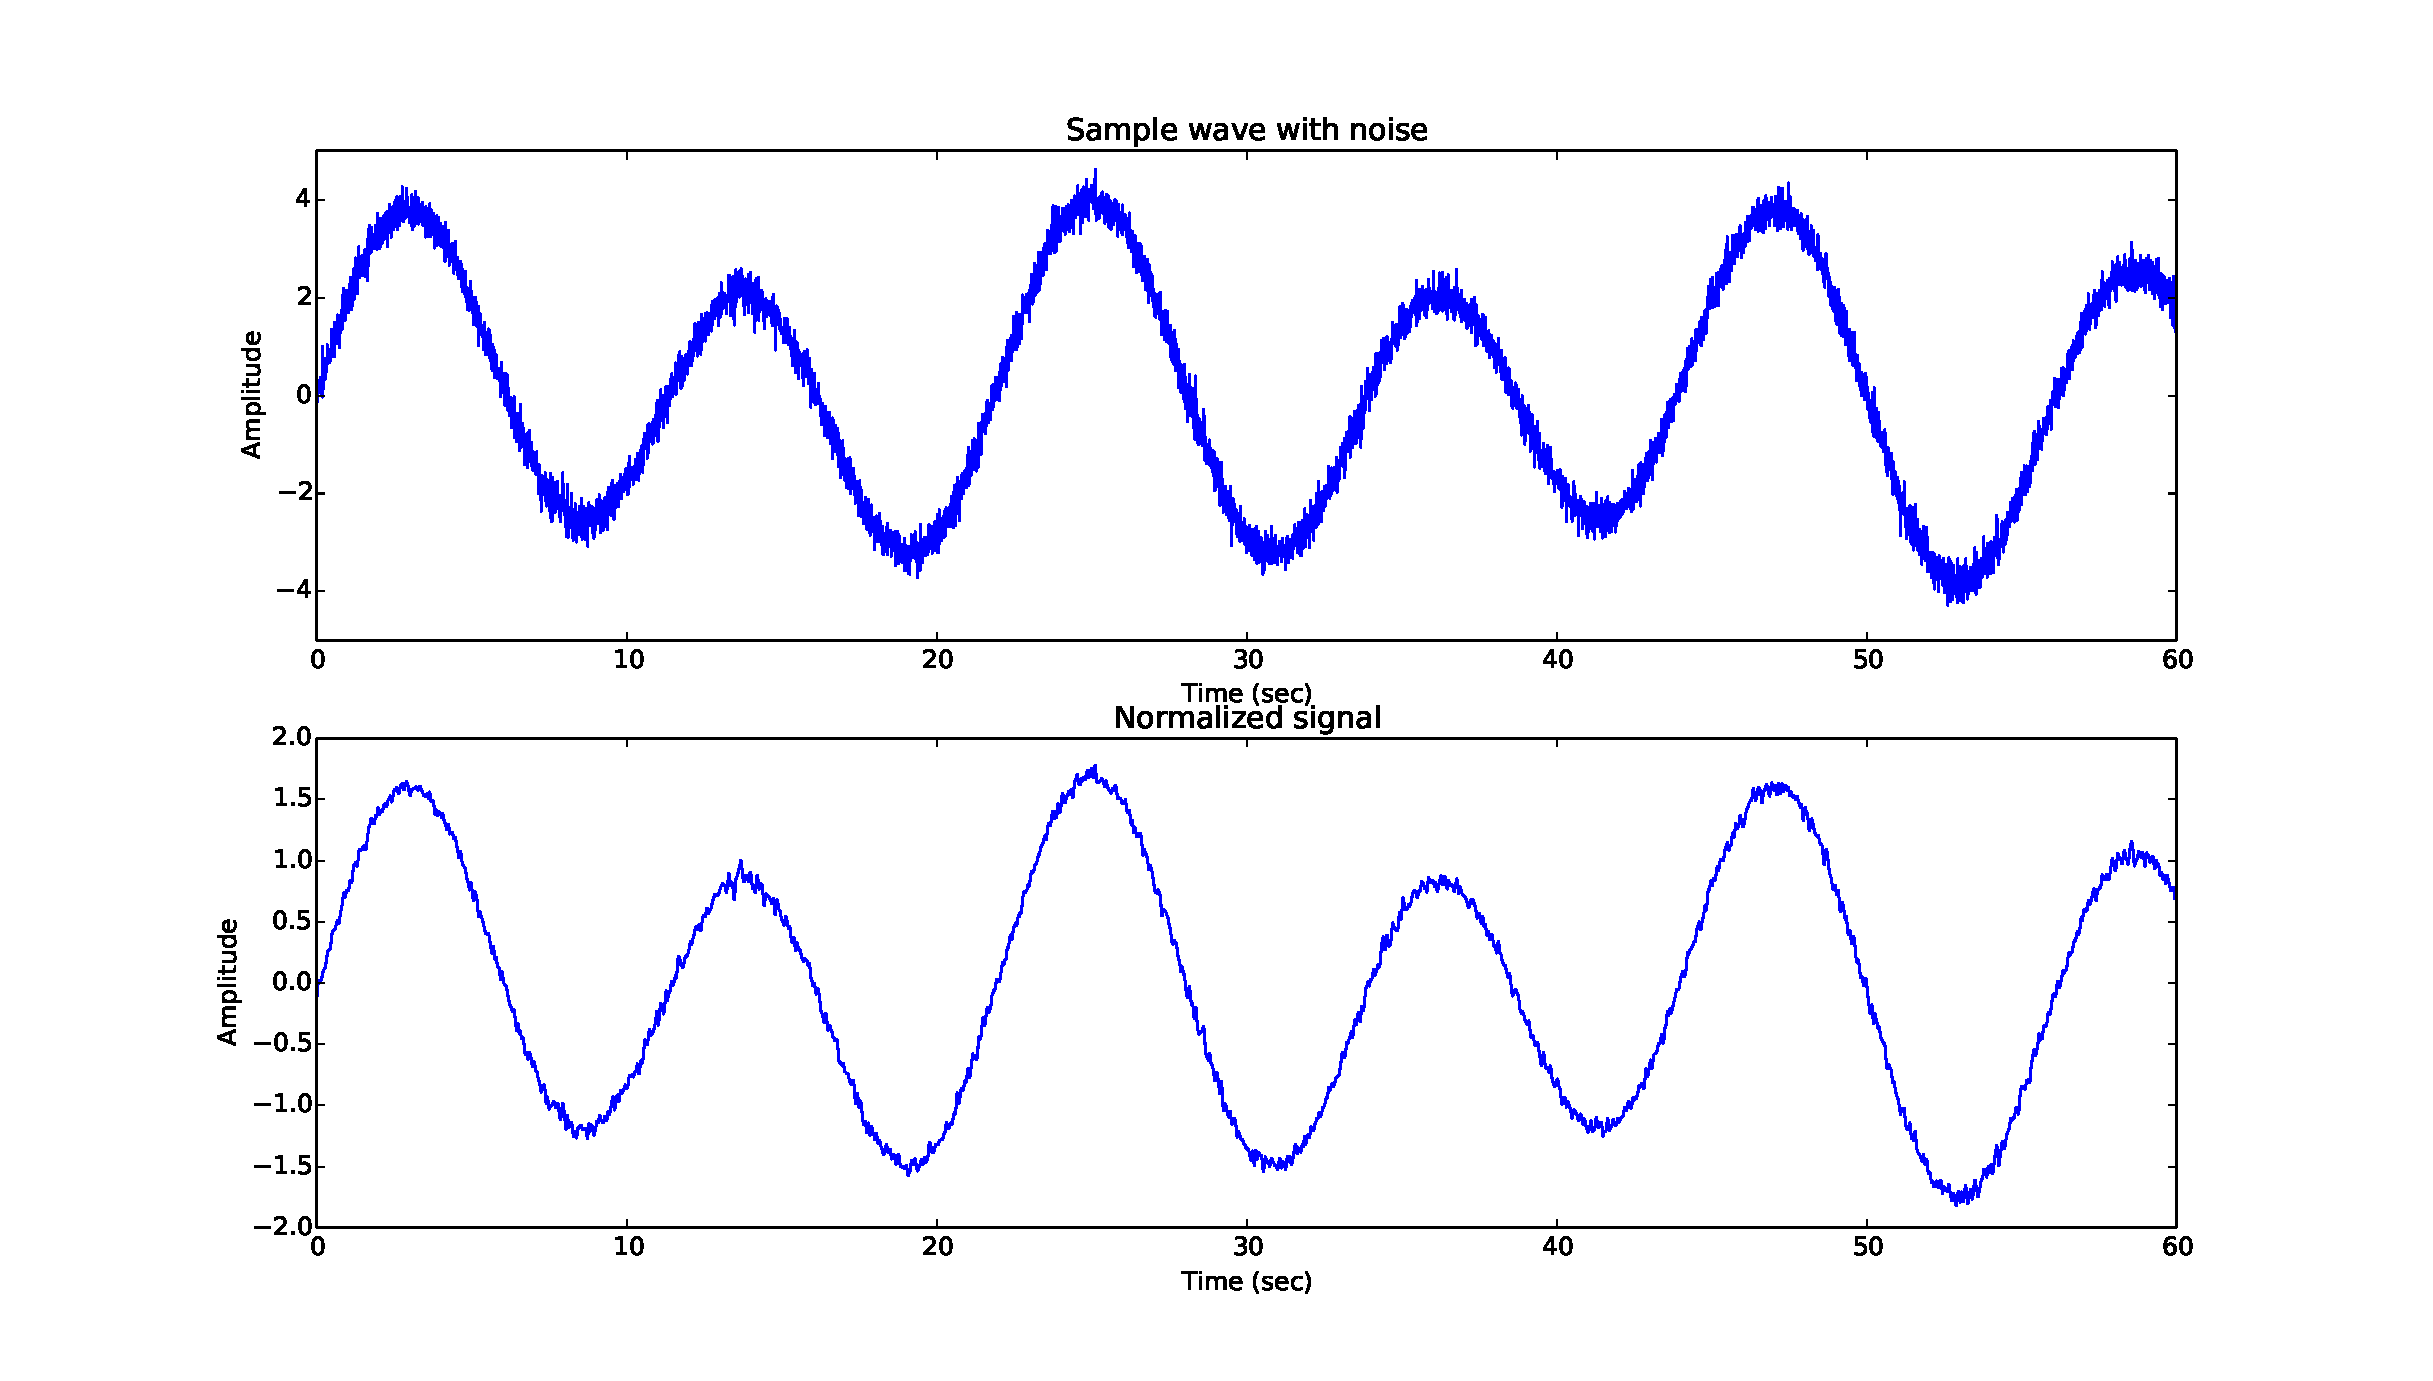
\includegraphics[width=15cm]{09_normalized.eps}
\caption{Sample sine wave normalized}
\label{fig:normalized}
\end{figure}

The best way to identify the missing fundamental frequency in a signal is to perform autocorrelation. Autocorrelation is a cross-correlation of a signal with itself. Mainly the autocorrelation yields repeating events from a signal. By definition for discrete time signal $x_n$ at time lag $j$, autocorrelation $R$ is

\begin{equation}
 R_{xx}(j) = \sum_{n}x_n\overline{x}_{n-j}
\end{equation}

Nevertheless one of the most computationally cheap ways to perform autocorrelation is do the inverse Fourier transform of the product of the discrete Fourier transform with the conjugate of the previously computed Fourier transform. Discrete Fourier transforms can be performed using FastFFT algorithm.

\begin{figure}[!ht]
\centering
  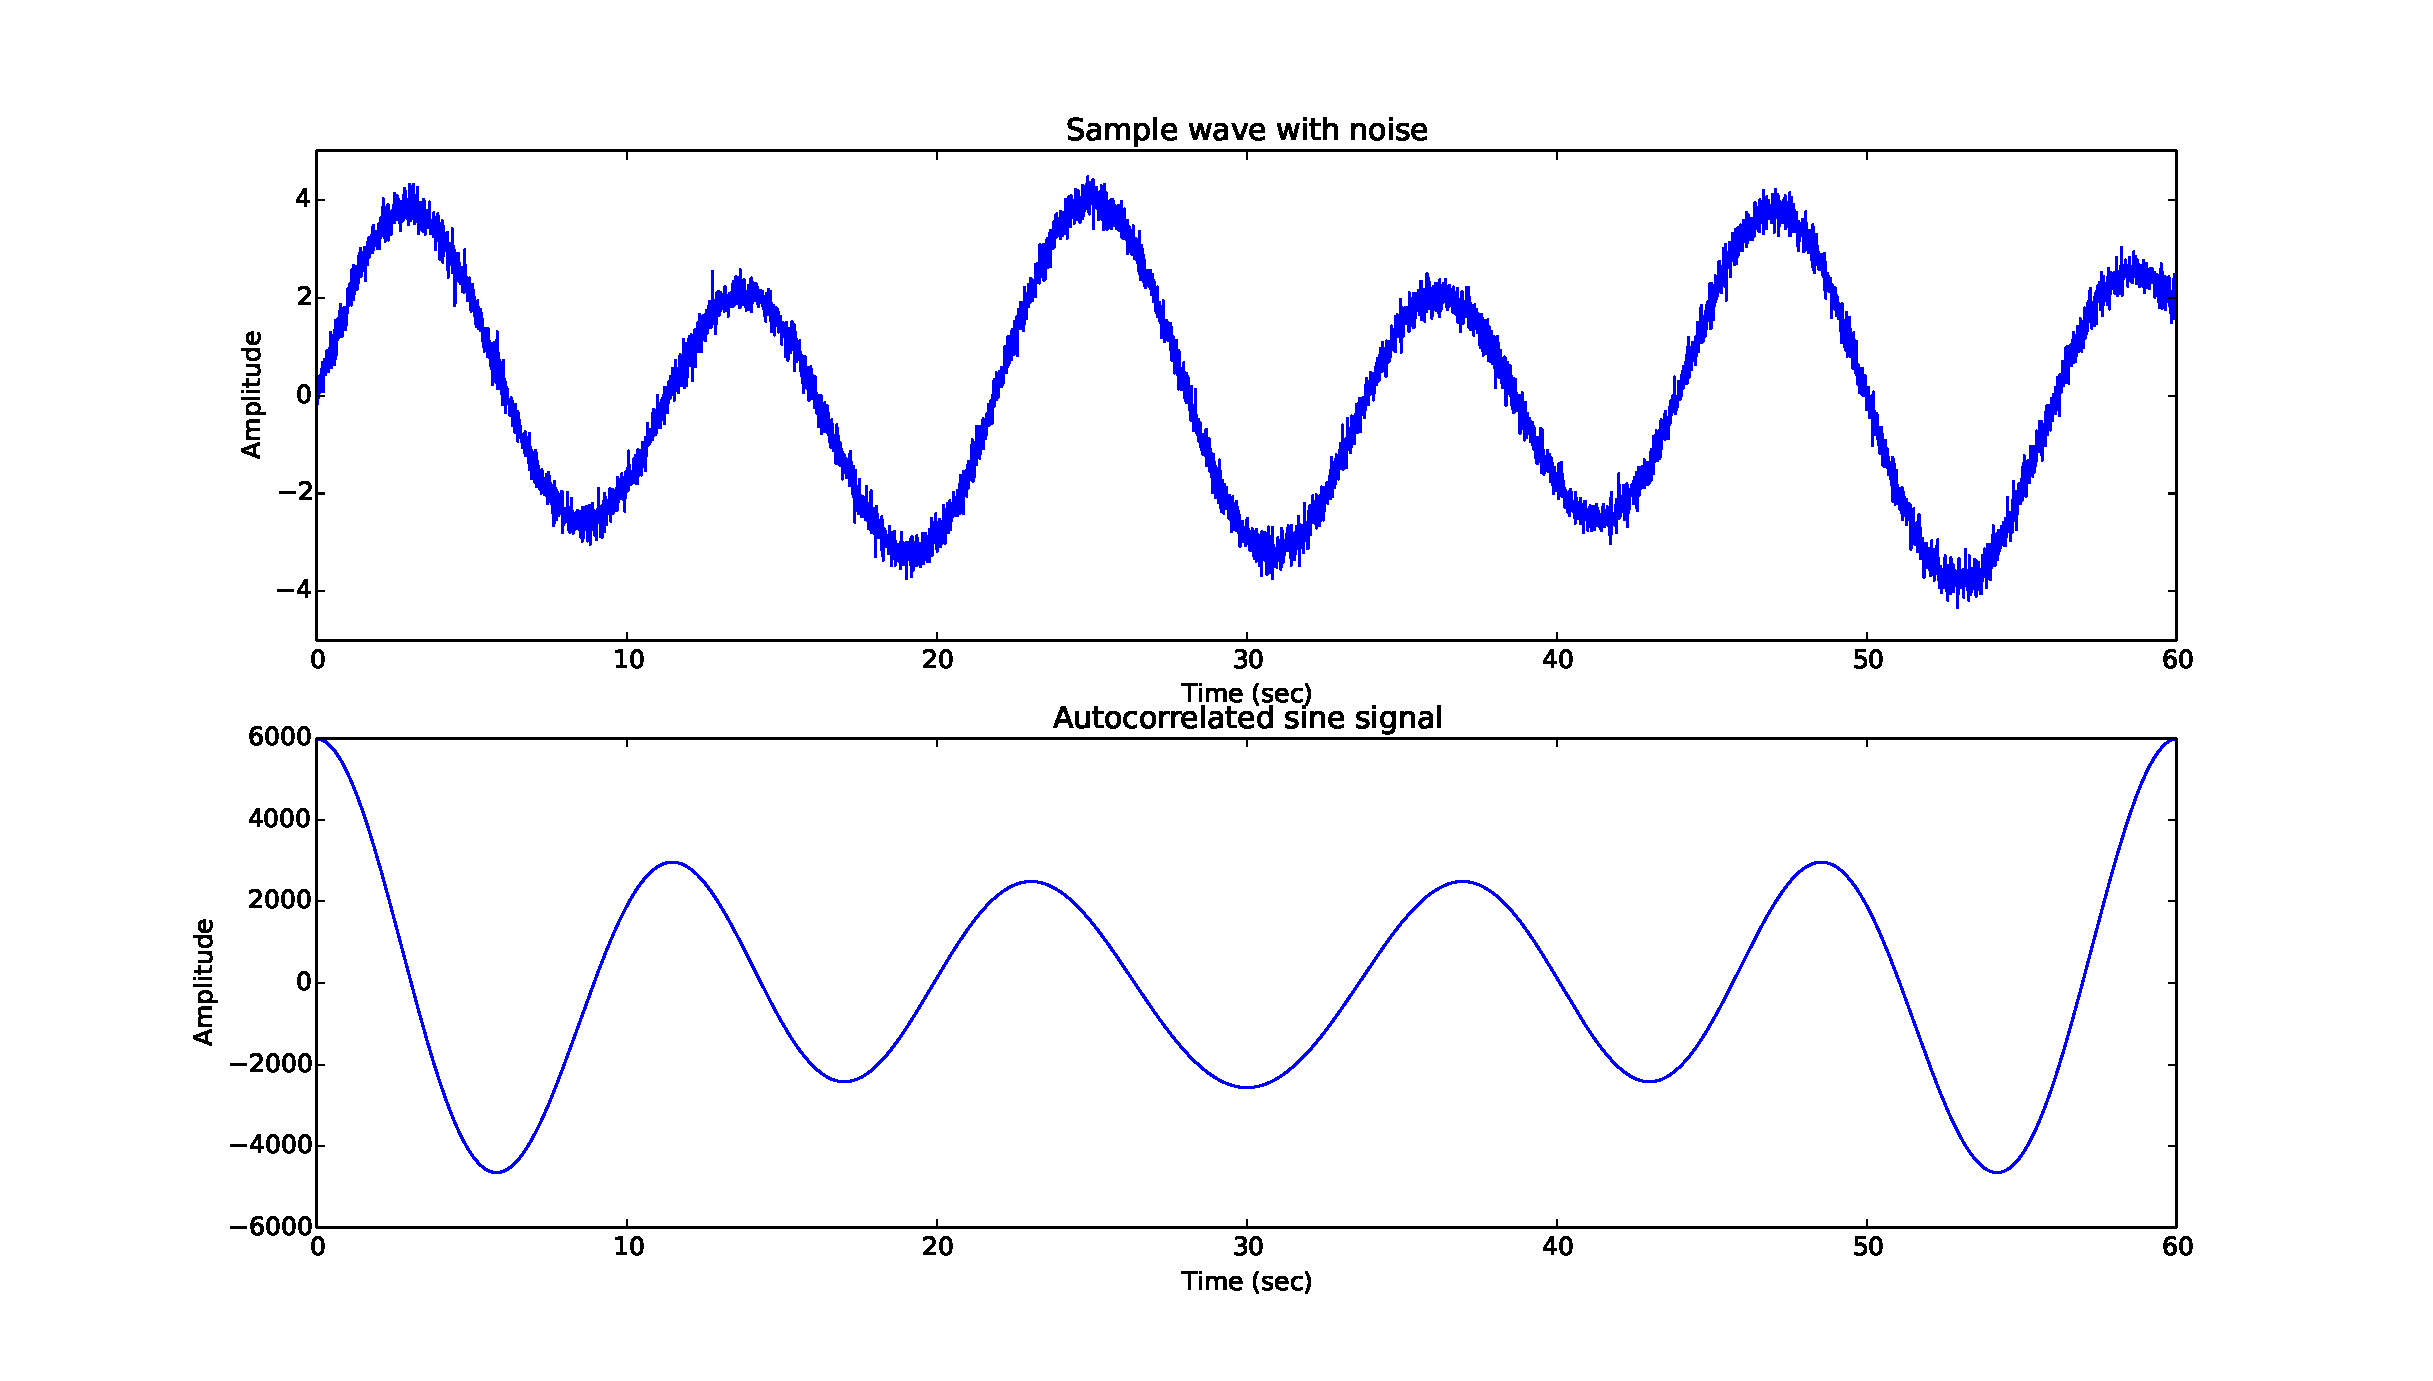
\includegraphics[width=15cm]{10_autocorrelation.eps}
\caption{The autocorrelation of the sine wave}
\label{fig:autocorrelation}
\end{figure}

All the manipulations performed till this point were done in time domain. In time domain one can see the changes that happen to a signal over time, whereas in frequency domain one can observe how much of the signal lies within each frequency band over a range of frequencies. Normally signals can be converted from one domain to the other using transformations like Fourier series, Fourier transform, Laplace Transform, Z transform. 

As previously mentioned Fourier transform performs a mathematical transformation from time to frequency domain and vice-versa. In engineering FFT (Fast Fourier Transform) algorithm is used widely due to its rapid computations. It factorizes the DFT (Discrete Fourier Transform) matrix into a product of sparse factors.  The DFT is defined by the Formula \eqref{eq:dft}.

\begin{equation} \label{eq:dft}
 X_k = \sum_{n=0}^{N-1} x_n e^{-i2\pi k\frac{n}{N}}, \qquad k= 0,\ldots , N-1
\end{equation}

Equation \eqref{eq:dft} has $O(N^2)$ complexity. In comparison, all known FFT algorithms require $\Theta (N \log N)$ operations, which represents a major improve in speed. FFT can also be used in computing Power Spectral Density (further used as PSD).

PSD shows how the variance of data is distributed over the frequency domain and represents a very useful tool to identify oscillatory signals in time series. On $x$ axis it represents the signal frequencies and on $y$ axis the amplitude. 

\begin{figure}[!ht]
\centering
  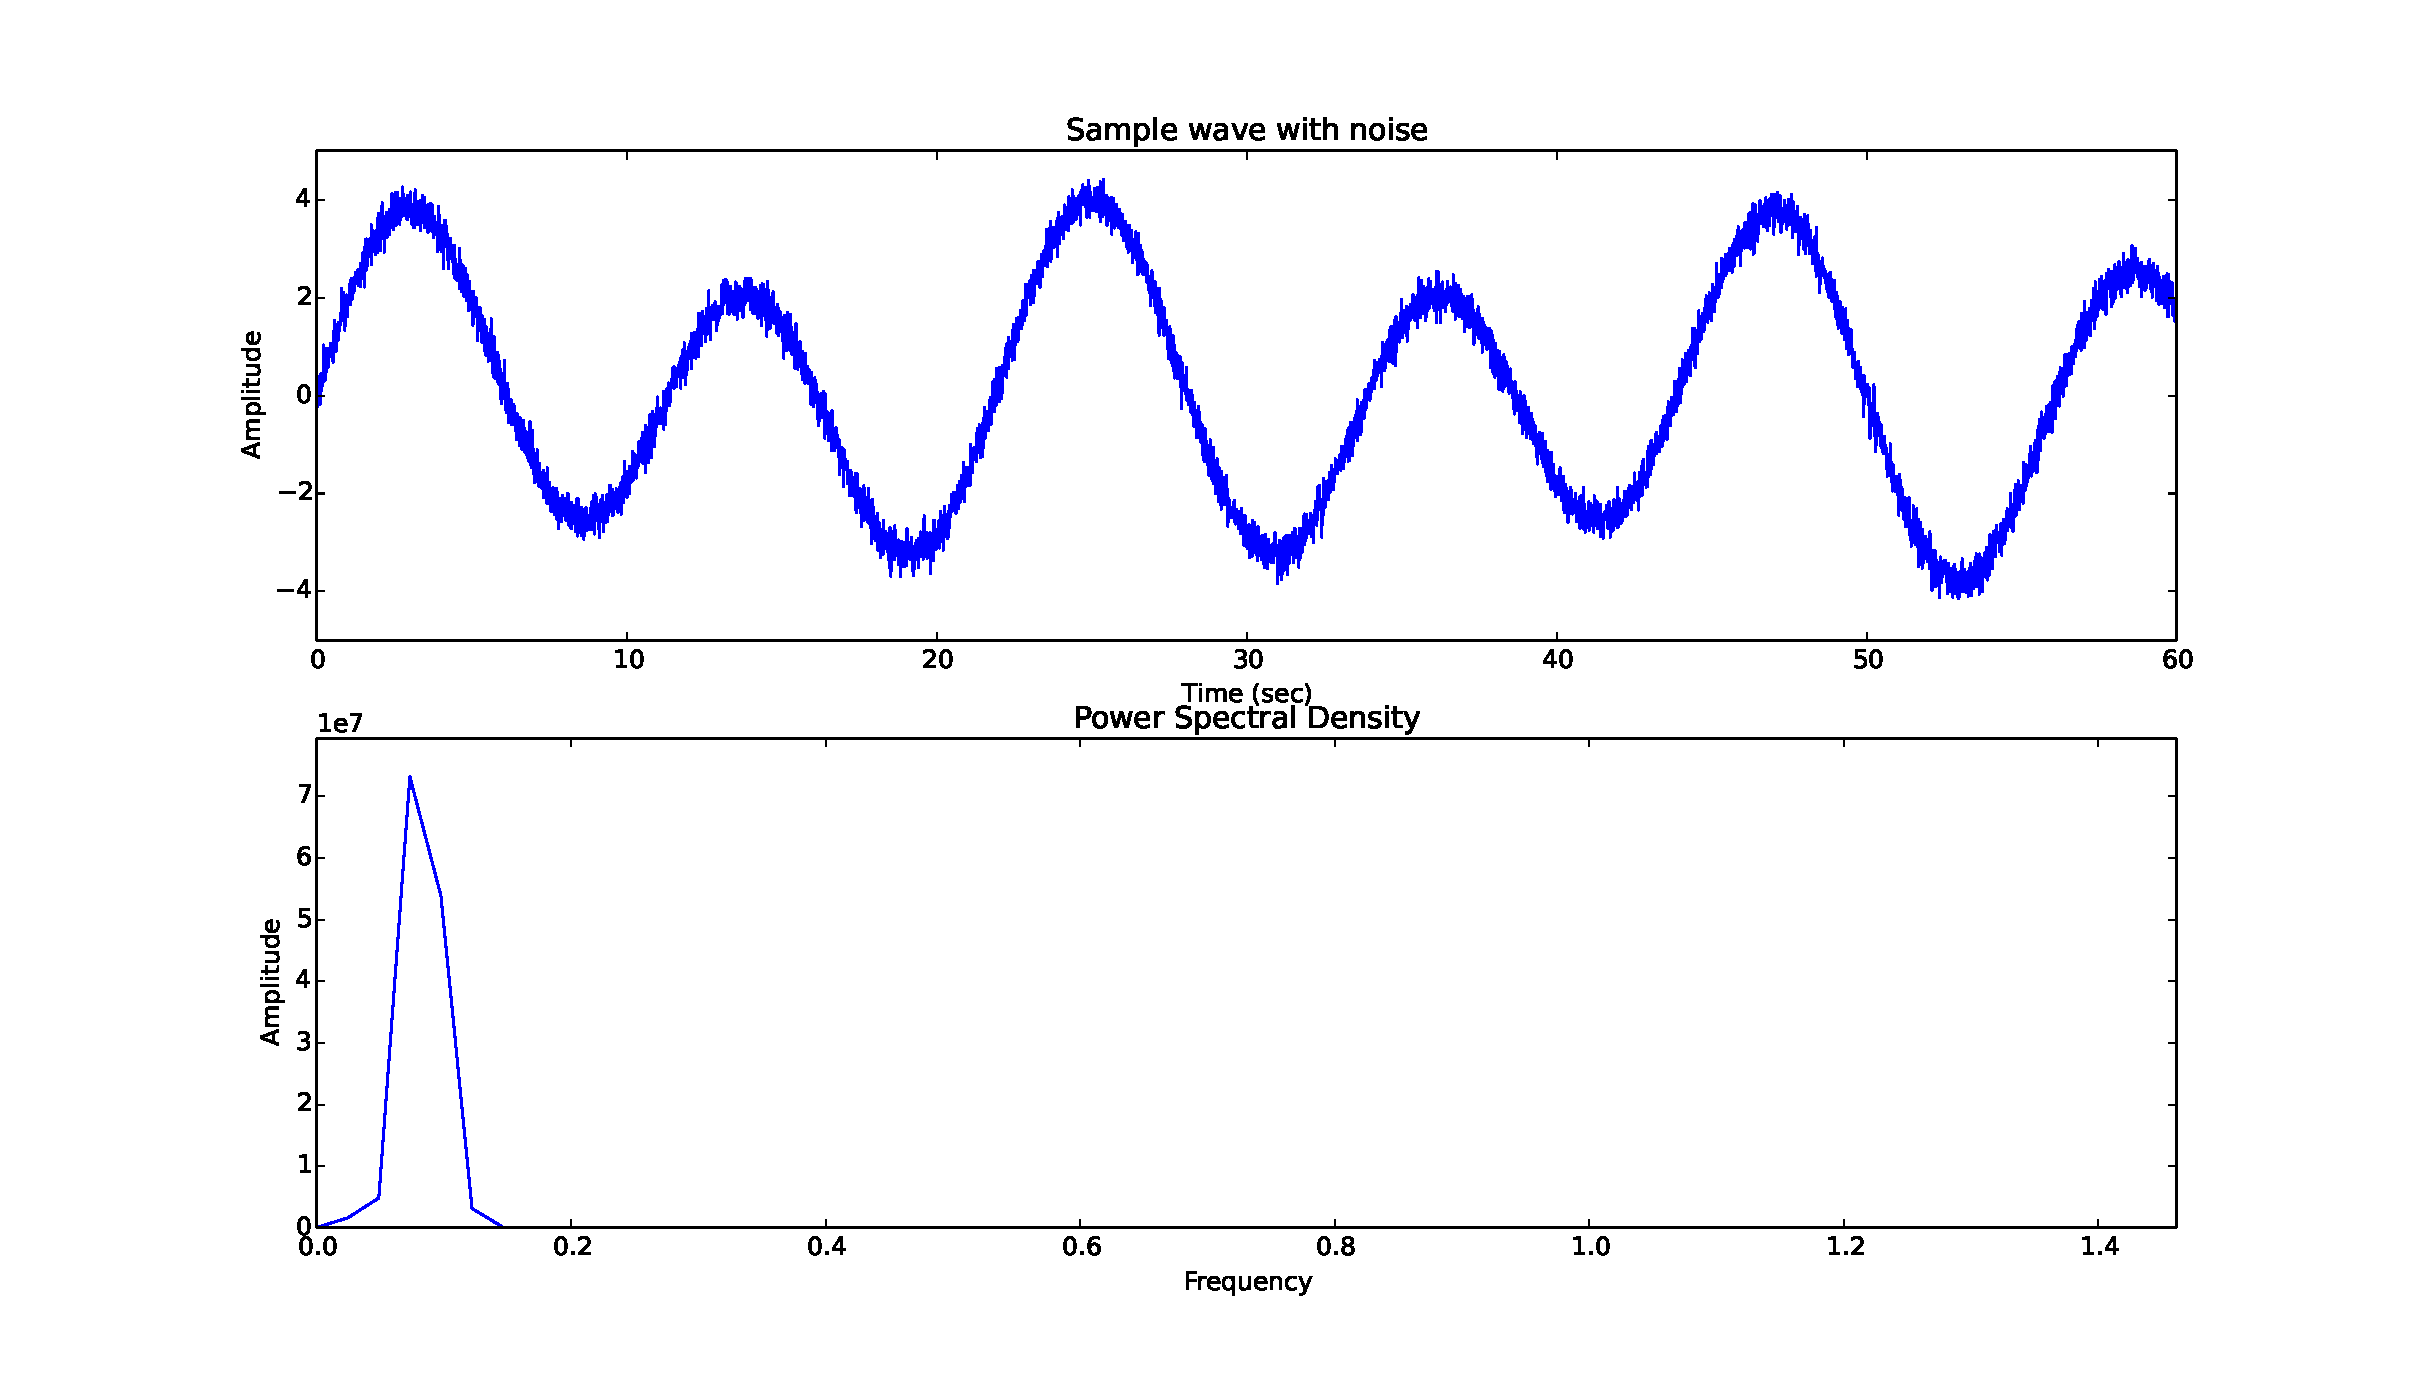
\includegraphics[width=15cm]{11_psd.eps}
\caption{Power Spectral Density of the signal}
\label{fig:psd}
\end{figure}

In Figure \ref{fig:psd} it is clearly seen a peak at about $0.05$ and a nearby point at $0.09$. Both points represent the initial frequencies that we used to generated the signal. 

To conclude DSP offered a variety of tools and algorithms to manipulate the initial noisy signal in order to achieve a concise representation with the most relevant information.

\subsubsection{Feature extraction and supervised learning}
In Machine Learning field one the most important aspect is considered feature extraction. The number of features and their quality are shaping the final result. The whole process of DSP was applied in order to 

\clearpage


